\documentclass[a4paper,11pt]{article}

\usepackage[utf8]{inputenc}
\usepackage[T1]{fontenc}    
\usepackage{lmodern}     
\usepackage{amsmath,amsthm,amssymb}
\usepackage{geometry}
\usepackage{graphicx}
\usepackage{xcolor} 
\usepackage{xspace}

\usepackage[french]{babel}
\usepackage{hyperref}    

% DEFINITIONS POUR LES THEOREMES
\theoremstyle{plain}
\newtheorem{thm}{Théorème}[section]
\newtheorem{prop}[thm]{Proposition}
\theoremstyle{definition}
\newtheorem{defi}[thm]{Définition}
\theoremstyle{remark}
\newtheorem*{rmk}{Remarque}
\newtheorem*{exe}{Exemple}



% COMMANDES PERSONNELLES
\newcommand{\ensemble}[1]{\mathbb{#1}}
\newcommand{\R}{\ensemble{R}}
\newcommand{\ie}{\textit{i.e.}\xspace}
\newcommand{\nom}[1]{\textsc{#1}\xspace}
\newcommand{\fermat}{\nom{Fermat}}


% DEFINITIONS POUR LE TITRE DU DOCUMENT
\title{Quelques remarques sur la vie de Pierre de \fermat}
\author{Votre Nom}

\begin{document}
\maketitle
\tableofcontents

\section*{Introduction}
Pierre de \fermat, né dans la première décennie du \textsc{xvii}\ieme siècle à Beaumont-de-Lomagne et mort le 12 janvier 1665 à Castres, est un magistrat et mathématicien français, surnommé \flqq le prince des amateurs\frqq. Il est en même temps un habile latiniste et helléniste. Il s'est aussi intéressé aux sciences physiques; on lui doit notamment le principe de \fermat en optique.

\begin{figure}
\centering
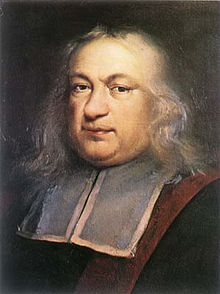
\includegraphics[width=0.2\textwidth]{fermat}
\caption{Pierre de \fermat}
% \label{fig:euler}
\end{figure}%


\begin{rmk}
Les éléments biographiques sont tirés de \url{http://fr.wikipedia.org/wiki/Pierre_de_Fermat}
\end{rmk}




\section{Quelques résultats mathématiques marquants}
\fermat partage avec \textsc{Viète}, dont il utilise les notations, et \textsc{Descartes}, avec qui il fut en conflit, la gloire d'avoir appliqué l'algèbre à la géométrie.

\textsc{D'Alembert} voyait dans ses travaux la première application du calcul infinitésimal. Il imagina, en effet, pour déterminer les tangentes, une méthode, dite \textit{de maximis et minimis}, qui le fait regarder comme le premier inventeur du calcul différentiel et le premier à utiliser des formules de dérivation.

\fermat contribue dans son échange épistolaire avec Blaise \textsc{Pascal} à élaborer les bases du calcul des probabilités, une mathématique du hasard que provoque l'étude du problème des partis du chevalier de Méré. Mais sa contribution majeure concerne la théorie des nombres et les équations diophantiennes. Auteur de plusieurs théorèmes ou conjectures dans ce domaine, il est au cœur de la \flqq théorie moderne des nombres\frqq.

\subsection{Les \flqq théorèmes de \fermat\frqq}
Il est très connu pour deux \flqq théorèmes\frqq:
\begin{itemize}
\item le \flqq petit théorème de Fermat\frqq;
\item le \flqq dernier théorème de Fermat\frqq (ce dernier n'était qu'une conjecture et l'est resté durant plus de trois siècles de recherches fiévreuses).
\end{itemize}



\begin{thm}[Petit théorème de \textsc{Fermat}]\label{theoreme.I}
Si $p$ est un nombre premier et $a$ un entier naturel non divisible par $p$, alors $a^{p-1}\equiv 1 \mod p$. 
\end{thm}
\begin{proof}
\fermat n'a pas fourni sa démonstration du théorème~\ref{theoreme.I}. Le 18 octobre 1640, il écrit à Frénicle de \textsc{Bessy}:
\begin{quotation}
\flqq Tout nombre premier mesure infailliblement une des puissances $-1$ de quelque progression que ce soit, et l'exposant de la dite puissance est sous-multiple du nombre premier donné $-1\dots$ Et cette proposition est généralement vraie en toutes progressions et en tous nombres premiers; de quoi je vous envoierois la démonstration, si je n'appréhendois d'être trop long.\frqq
\end{quotation}
\end{proof}

% Gottfried Wilhelm \textsc{Leibniz} a rédigé en 1683 une démonstration qu'il ne publie pas. Leonhard \textsc{Euler} a démontré le théorème en 1736 par les mêmes arguments. Il communique cette preuve le 2 août 1736 à l’Académie de Saint-Pétersbourg et publie cette première démonstration en 1741. Elle repose sur une récurrence et l'utilisation du développement du binôme.

\begin{thm}[Dernier théorème de Fermat]
Lorsque $n$ est un entier strictement supérieur à $2$, il n'existe pas d'ensemble d'entiers strictement positifs $x$, $y$, $z$ vérifiant l'équation 
\[
x^n + y^n = z^n.
\]
\end{thm}

\begin{rmk}
Ce théorème fut démontré par le mathématicien anglais Andrew \textsc{Wiles} de l'Université de Princeton, avec l'aide de Richard \textsc{Taylor}. Après une première présentation en juin 1993, puis la découverte d'une erreur et un an de travaux supplémentaires, la preuve fut finalement publiée en 1995 dans \emph{Annals of Mathematics}. 

Pierre de \fermat lui-même annotait dans la marge de son exemplaire des Arithmétiques qu’il en avait découvert une démonstration vraiment remarquable, mais manquait de place pour la donner à cet endroit:
\begin{quotation}
\flqq J'ai trouvé une merveilleuse démonstration de cette proposition, mais la marge est trop étroite pour la contenir.\frqq
\end{quotation}
Il semble assez improbable que Pierre de \fermat ait réellement réussi à démontrer ce théorème dans le cas général; en effet, la démonstration réalisée par Andrew \textsc{Wiles} (même si le dernier théorème de \fermat n'en est qu'un corollaire) utilise des outils mathématiques d'une grande complexité dont on ne semble guère pouvoir se passer. Compte tenu des connaissances de son époque, \fermat ne pouvait pas les soupçonner.
\end{rmk}







\subsection{Les nombres de \fermat}
Un nombre de \fermat est un entier naturel qui peut s'écrire sous la forme $2^{2^n}+1$, avec $n$ entier. Le $n$-ème nombre de \fermat est noté $F_n$.

Ces nombres doivent leur nom à \fermat qui émit la conjecture que tous ces nombres étaient premiers. Cette conjecture se révéla fausse, $F_5$ étant composé, de même que tous les nombres de \fermat jusqu'à $F_{32}$. On ne sait pas si les nombres à partir de $F_{33}$ sont premiers ou composés. Les seuls nombres de Fermat premiers connus sont donc $F_0$, $F_1$, $F_2$, $F_3$ et $F_4$.


\subsubsection{Propriétés}
La suite des nombres de Fermat possède plusieurs relations de récurrence. Par exemple, si $n\ge2$, on a
\[
F_n=(F_{n-1}-1)^2+1
\qquad\text{ou}\qquad
F_n=F_{n-1}^2-2(F_{n-2}-1)^2
\]
ou encore, avec des produits de nombres de \fermat,
\[
F_n=2+\prod_{i=0}^{n-1}F_i
\qquad\text{ou}\qquad
F_n=F_{n-1}+2^{(2^{n-1})}\prod_{i=0}^{n-2}F_i.
\]

On en déduit le théorème 
\begin{thm}[\textsc{Goldbach}]
Deux nombres de \fermat distincts sont premiers entre eux.
\end{thm}


        

Soit $D(n, b)$ le nombre de chiffres utilisés pour écrire $F_n$ en base $b$, alors\footnote{Les crochets désignent la fonction partie entière et $\log_b$ le logarithme de base $b$.} 
\begin{align}
D(n,b)&= \lfloor 1+\log_b\left( 2^{2^n}+1 \right) \rfloor\\
    &\approx \lfloor 1+\log_b\left( 2^{2^n}\right) \rfloor\\
	&=1+\lfloor 2^n\log_b(2)\rfloor.
\end{align}
Par exemple, en notation décimale, 
\begin{enumerate}
\item $F_0=3$ et $D(0,10)=1$,
\item $F_1=5$ et $D(1,10)=1$, 
\item $F_2=17$ et $D(2,10)=2$, 
\item $F_3=257$ et $D(3,10)=3$, 
\item $F_4=65537$ et $D(4,10)=5$, 
\item $F_5=4294967297$ et $D(5,10)=10$.
\end{enumerate}


La raison historique de l'étude des nombres de \fermat est la recherche de nombres premiers. \fermat connaissait déjà la proposition suivante
\begin{prop}
Soit $k$ un entier strictement positif, si le nombre $2^k + 1$ est premier alors $k$ est une puissance de $2$.
\end{prop}
\begin{proof}
Il existe deux entiers $a$ impair et $b$ tels que $k = a 2^b$. En posant $c = 2^{2^b}$, on dispose alors des égalités suivantes
\[
1+2^k =1 + c^a= (1 + c)\sum_{i=0}^{a-1} (-1)^i c^i,
\]
qui montrent que $1 + c$ est un diviseur du nombre premier $1 + 2^k$ et donc lui est égal, si bien que $k = 2^b$.
\end{proof}
Fermat a conjecturé (erronément) que la réciproque était vraie et il a montré que $F_n$ est premier pour $n=0,1,2,3,4$. Actuellement, on ne connaît que cinq nombres de \fermat premiers, ceux cités ci-dessus.
        
\subsubsection{Factorisation des nombres de \fermat composés}
\[
\begin{array}{|c|c|c|c|}
\hline
F_n&\text{$D(n,10)$}&\text{Nombre de facteurs}&\text{Facteurs}\\
\hline
5	&10		&2	&3\text{ et }7\\
\hline
6	&20		&2	&6\text{ et }14\\
\hline
7	&39		&2	&17\text{ et }22\\
\hline
8	&78		&3	&16\text{ et }62\\
\hline
9	&155	&3	&7,\ 49\text{ et }99\\
\hline
10	&309	&4	&8,\ 10,\ 40\text{ et }252\\
\hline
11	&617	&5	&6,\ 6,\ 21,\ 22\text{ et }564\\
\hline
\end{array}
\]


\end{document}